\chapter{کنترل اجماع ربات‌‌ها}
%\thispagestyle{empty}

\section{مقدمه}
این فصل را می‌توان مهم‌ترین بخش این پروژه دانست که هدف آن کنترل سیستم‌های چند عاملی\LTRfootnote{Multi-agent systems} به صورت دسته‌ای\LTRfootnote{Platoon} از ربات‌هاست، به طوری که رهبر\LTRfootnote{Leader} دسته را دنبال کنند. در ادبیات سیستم‌های چند عاملی به هر خودرو یا ربات، عامل گفته می‌شود. همچنین همانطور که در ادامه خواهیم دید، یک خودرو فرضی نیز می‌تواند به عنوان رهبر در نظر گرفته شود. در سیستم‌های چند عاملی، هر عامل با داشتن اطلاعات عامل‌های دیگر، که می‌تواند بین یک تا تمام عامل‌های دیگر باشد، رهبر را دنبال می‌کند. در نتیجه، تمامی عامل‌ها درباره اینکه رهبر در کجا قرار دارد به اجماع\LTRfootnote{Consensus} برسند. به همین دلیل به الگوریتم‌های انجام دهنده این عمل، الگوریتم اجماع می‌گویند.

الگوریتم‌های اجماع تحت تاثیر ارتباطات بین عامل‌ها هستند و می‌توان با توجه به اینکه کدام ربات‌ها با هم داده تبادل می‌کنند، گراف ساده جهت‌داری\LTRfootnote{Simple directed graph} رسم نمود. به این منظور هر عامل را به یک راس\LTRfootnote{Vertex} و هر ارتباط را یک یال\LTRfootnote{Edge} جهت‌دار که از عامل فرستنده یال خارج و به عامل گیرنده وارد می‌شود، نسبت داد. همچنین، دور به طول‌ یک، یالی که از یک راس به خودش وارد می‌شود، و تعداد بیشتر از یک یال بین دو راس مشخص وجود ندارد. هر گراف را می‌توان به نحوه‌های مختلفی، همچون ماتریس مجاورت\LTRfootnote{Adjacency matrix} و لیست مجاورت\LTRfootnote{Adjacency list} نمایش داد. در پروژه با توجه به ادامه کار و نیازمان، از ماتریس مجاورت استفاده شده است که دلیل آن را در ادامه خواهیم دید.

\section{گراف اجماع}
گراف اجماع تاثیر بسیار زیادی بر پروژه و عملکرد آن دارد. هر یال (ارتباط)، به دلیل اضافه کردن محاسبات، شامل هزینه زمانی است و باعث بیشتر شدن زمان نمونه برداری می‌شود. از طرفی در صورت قطعی موقت ارتباط، نباید عامل ارتباط خود با دسته را به طور کامل از دست ندهد. در نتیجه مبحثی که پیش می‌آید این است که گرافی را طوری طراحی کنیم که در صورت قطع یک سری از ارتباطات تضمین شود هیچ عاملی ارتباطش را با دسته از دست نمی‌دهد. در این راستا از مباحث نظریه گراف بهره می‌بریم.

\subsection{عدد همبندی یالی}\label{se edge connectivity}

 در ادبیات نظریه گراف \verb|E| مجموعه یال‌ها و \verb|V| مجموعه راس‌ها در نظر گرفته می‌شود. فرض کنید
$ G = (V,E)$
  گرافی همبند باشد و 
$T \subseteq E$
باشد به طوری که 
$G - T$
ناهمبند باشد. در این صورت \verb|T| را یک مجموعه برشی یالی (برش یالی)\LTRfootnote{Edge cut (set)} گویند.

مجددا فرض کنید 
$ G = (v,E)$
یک گراف ساده باشد، آنگاه \verb|G| را \verb|k|-همبند یالی\LTRfootnote{k-edge connected} هرگاه 
$|V| > 1$
 و برای هر 
$T \subseteq E$
 که 
$|T| < k$
 باشد، 
$G - T$
گرافی همبند باشد. از تعریف می‌توان نتیجه گرفت که اگر گرافی \verb|k+1|-همبند یالی باشد آنگاه \verb|k|-همبند یالی است. در نتیجه بزرگترین مقدار \verb|k|، که گراف \verb|G| به ازای آن \verb|k|-همبند یالی باشد ارزش دارد و آن را (عدد) همبندی یالی\LTRfootnote{Edge connectivity} گراف \verb|G| گویند و با 
$k^\prime(G)$
نمایش می‌دهند.

برای به دست آوردن حد بالای عدد همبندی یالی، یکی از راس‌هایی که دارای کمترین درجه\LTRfootnote{degree} در گراف است را در نظر بگیرید. درجه این راس را با 
$\delta(G)$
نمایش می‌دهند. اگر تمام یال‌های وارده به این راس را حذف کنیم، به یک راس ایزوله می‌رسیم و چون در تعریف عدد همبندی یالی شرط وجود بیشتر از یک راس در گراف بود، گراف ناهمبند می‌شود زیرا مسیری بین این راس و راس‌های دیگر وجود ندارد. در نتیجه اثبات ذکر شده می‌توان نوشت:
\begin{equation}\label{eq k-edge delta}
k^\prime(G) \leq \delta(G)
\end{equation}

مزیت رابطه \ref{eq k-edge delta} در این است که به راحتی دید خوبی از بیشترین مقدار ممکن برای عدد همبندی یالی پیدا می‌کنیم.

اهمیت عدد همبندی یالی در گراف اجماع این است که اگر تعداد 
$k^\prime(G) - 1$
 ارتباط قطع شود، ارتباط غیر مستقیم دسته عامل‌ها همچنان حفظ می‌شود و هر یک می‌دانند که باید در چه موقعیتی قرار گیرند. پس هر چه قدر عدد همبندی یالی بزرگتر شود، ارتباط بین عامل‌ها مقاوم‌تر تلقی می‌شود.

\subsection{کمینه‌ترین گراف اجماع}\label{sec least formation graph}

همانطور که صحبت شد، بیشتر شدن یال‌ها موجب افزایش زمان نمونه برداری می‌شود. از طرفی بزرگ بودن عدد همبندی یالی نیز به عنوان معیاری از مقاوم بودن گراف در برابر قطع شدن ارتباط‌ها می‌باشد. طبق تعاریف انجام شده در قسمت \ref{se edge connectivity}، می‌توان گفت که اضافه کردن یال عدد همبندی یالی را کاهش نمی‌دهد و در بعضی از شرایط موجب افزایش آن می‌شود. پس در تشکیل گراف اجماع، نکته قابل توجه، انتخاب برقرار کردن یا نکردن ارتباط بین هر دو عامل است به طوری که کمینه‌ترین ارتباط با توجه به عدد همبندی یالی مورد نظرمان برقرار شود.

در حالت ایده‌آل، اگر اطمینان داده شود که هیچ ارتباطی قرار نیست از دست رود، می‌توان عدد همبندی یالی را برابر یک در نظر گرفت. یک درخت\LTRfootnote{Tree} با ریشه\LTRfootnote{Root} رهبر، کمینه‌ترین ارتباط را به ازای 
$k^\prime(G) = 1$ 
برقرار می‌کند. منظور از کمینه‌ترین ارتباط در این حالت، این است که اولا گراف ضعیفا همبند\LTRfootnote{Weakly connected} باشد، به این معنا که با جایگزینی یال‌های جهت‌دار با یال بی‌جهت بین هر دو عامل (راس)، مسیری وجود داشته باشد. از طرفی منظور از کمینه بودن، این است که با حذف هر ارتباط، همبندی و در نتیجه ارتباط غیر مستقیم با رهبر از دست برود. در صورت وجود دور در گراف، می‌توان یکی از یال‌ها را حذف نمود و هنوز ارتباط بین عامل‌ها حفظ شود. در نتیجه گراف ما نباید دور داشته باشد. به گراف بدون دور همبند، درخت گفته می‌شود. همچنین به گرافی کمینه‌تر از درخت نمی‌شود رسید زیرا در صورت قطع ارتباط، بین هر دو عامل، عامل فرزند\LTRfootnote{Child}، راسی که ارتباط به آن وارد شده، و فرزندانش ارتباط خود را با والد\LTRfootnote{Parent}، راسی که ارتباط از آن خارج شده، و در نهایت رهبر از دست می‌دهند.

در حالتی که بخواهیم شبکه گراف، بیشترین مقاومت را نسبت به قطعی ارتباطات داشته باشد، یا به عبارتی به بیشترین مقدار ممکن برای عدد همبندی یالی برسیم، به طوری که گراف کمینه هم باشد، باید شبکه ارتباطات را به صورت گراف کامل ایجاد کرد. در ادامه ادعای بالا اثبات می‌شود.

تعداد عامل‌ها را برابر با \verb|n| می‌گیریم. پس داریم:
\begin{equation}
|V| = n
\end{equation}

با توجه به اینکه گراف ساده است پس حداکثر، از هر راس به تمامی رئوس دیگر می‌توان یال داشت. در نتیجه اگر همه رئوس به هم متصل باشند یا به عبارتی، درجه همه رئوس برابر با 
$n-1$
 باشد، آنگاه گراف کامل است و گراف کامل \verb|n| راسی را با 
$K_n$ 
نشان می‌دهیم. در نتیجه داریم:
\begin{equation}\label{eq delta max}
\delta(K_n) = n-1
\end{equation}

از روابط \ref{eq k-edge delta} و \ref{eq delta max} می‌توان نتیجه گرفت که:
\begin{equation}\label{eq connectivity max}
k^\prime(K_n) \leq n-1
\end{equation}

پس اگر گراف کامل نباشد، یعنی یک راسی وجود دارد که از آن به همه رئوس دیگر، یال وجود ندارد پس درجه آن راس کمتر از 
$n-1$
 و در نتیجه 
$\delta(G) < n-1$ 
خواهد بود. مجددا با توجه به رابطه \ref{eq k-edge delta}، می‌توان گفت که 
$k^\prime(G) < n-1$
خواهد بود. حال اگر اثبات شود که 
\begin{equation}\label{eq edge complete graph}
k^\prime(K_n) = n-1
\end{equation}
 
می‌توان نتیجه گرفت که به ازای یک 
$n-1$ 
ثابت به عنوان تعداد رئوس یک گراف ساده، به بیشترین مقدار ممکن برای عدد همبندی یالی می‌رسیم، اگر و فقط اگر آن گراف، کامل باشد.

برای اثبات رابطه \ref{eq edge complete graph}، از برهان خلف استفاده می‌کنیم. فرض کنید رابطه برقرار نباشد پس با توجه به رابطه \ref{eq connectivity max}، 
$k^\prime(K_n) < n-1$
است، زیرا از بالا محدود شده است. پس طبق تعریف، دو راس 
$\exists u,v \in V(K_n)$ 
وجود دارند، به طوری که با حذف کمتر از 
$n-1$
یال، گراف ناهمبند می‌شود. حال مسیر 
$uv$ 
و تمام مسیرهای 
$uwv$ 
را در نظر بگیرید به این صورت که \verb|w| رئوس دیگر گراف 
$K_n$
باشد. برای \verb|w|، 
$n-2$ 
انتخاب داریم. پس تعداد کل مسیرهای ذکر شده برابر 
$n-1$ 
است و همگی از هم مستقل یالی می‌باشند. به این معنی که هیچ یالی در این مسیرها تکرار نشده است. در نتیجه وجود مجموعه‌ یال‌هایی که تعداد آن‌ها کمتر از 
$n-1$ 
باشد و باعث شوند همگی این مسیرها از بین روند تا درنهایت بین دو راس \verb|u| و \verb|v| هیچ مسیری نباشد، تناقض است. پس فرض خلف باطل و حکم ثابت می‌شود. در نتیجه، قوی‌ترین گراف برای تشکیل ارتباطات و همچنین کمینه‌ترین آن، گراف کامل می‌باشد. حال به تشکیل گراف اجماع می‌پردازیم.

\subsection{تشکیل گراف اجماع}
در این پروژه آزمایشات بر روی 4 ربات انجام شده است که رهبر مجازی است و تنها 3 ربات وجود فیزیکی دارند. با توجه به بخش \ref{sec least formation graph} می‌توان گفت در صورتی که تنها ارتباط دو طرفه بین عامل رهبر و بقیه عامل‌ها برقرار شود به کمینه‌ترین گراف اجماع خواهیم رسید که دارای 3 یال خواهد بود. با وجود نکته بالا، به دلیل اینکه گراف مقاوم‌تری داشته باشیم، از گراف کامل $K_4$ استفاده شده است. 


\section{الگوریتم اجماع}
در این پایان‌نامه از دینامیک تک انتگرال‌گیر\LTRfootnote{Single integrator} برای ارتباط بین موقعیت‌های ربات‌ها استفاده شده است. می‌توان این الگوریتم‌ را به صورت زیر در نظر گرفت:
\begin{equation}\label{eq platoon sum}
\dot{x}_i = -\sum_{j=1}^{n} a_{ij}(x_i-x_j)
\end{equation}

که در آن $a_{ij} = 1$ اگر از راس \verb|j| به \verb|i| یالی وارد شده باشد. در غیر این صورت $a_{ij} = 0$ خواهد بود. به عنوان مثال اگر داشته باشیم:
\begin{equation}
\dot{x}_3 = -(x_3-x_1)-(x_3-x_2)
\end{equation}

به این معنی است که داده عامل 1 و 2 به 3 می‌رسد. اگر $x$ را موقعیت تعریف کنیم، اثبات می‌شود که تحت ماتریس‌بندی خاصی با گذشت زمان، موقعیت عامل‌ها به هم خواهند رسید. در نتیجه اگر یکی از ربات‌ها رهبر باشد، بقیه به موقعیت آن خواهند رسید.

علاوه بر دینامیک تک انتگرال‌گیر، مدل‌های دو انتگرال‌گیر\LTRfootnote{Double integrator}، مدل خطی یا غیر خطی نیز می‌توانند استفاده گردند. برای سادگی مدل تک انتگرال‌گیر در این پایان‌نامه استفاده شده است.

 اگر ماتریسی که با $a_{ij}$ ساخته می‌شود را $A$ نامیم، ماتریس لاپلاسین\LTRfootnote{Laplacian matrix} آن به صورت زیر تعریف می‌شود:
\begin{equation}\label{eq L = D - A}
L(A) = D(A) - A
\end{equation}
 
 که در آن $(A)D$ ماتریس درجه گراف $A$ است که در آن مجموع درجات هر راس بر روی قطر اصلی، متناظر با سطر آن راس، نوشته می‌شود.
 برای سادگی ماتریس‌های $D(A)$ و $L(A)$، با $D$ و $L$ نوشته خواهند شد. می‌توان رابطه \ref{eq platoon sum} را به فرم ماتریسی، به صورت زیر نوشت:
\begin{equation}\label{eq x. = -Lx}
	\dot{x} = -Lx
\end{equation}

که نتیجه می‌دهد:
\begin{equation}\label{eq x = elt x}
	x(t) = e^{-Lt}x(0)
\end{equation}

در این پروژه، با توجه به استفاده از ماتریس کامل به عنوان گراف اجماع برای ارتباط 4 ربات داریم:
\begin{equation}
	A = K_4 = 
	\begin{bmatrix}
	0~~~~1~~~~1~~~~1 \\
	1~~~~0~~~~1~~~~1 \\
	1~~~~1~~~~0~~~~1 \\
	1~~~~1~~~~1~~~~0
	\end{bmatrix}
\end{equation}

که در نتیجه آن ماتریس لاپلاسین با توجه به رابطه \ref{eq L = D - A} به صورت زیر محاسبه می‌گردد:
\begin{equation}\label{eq L example}
	L = D - A = 
	\begin{bmatrix}
	3~~~~0~~~~0~~~~0 \\
	0~~~~3~~~~0~~~~0 \\
	0~~~~0~~~~3~~~~0 \\
	0~~~~0~~~~0~~~~3
	\end{bmatrix}
	-
	\begin{bmatrix}
	0~~~~1~~~~1~~~~1 \\
	1~~~~0~~~~1~~~~1 \\
	1~~~~1~~~~0~~~~1 \\
	1~~~~1~~~~1~~~~0
	\end{bmatrix}
	=
	\begin{bmatrix}
	~~3~~~-1~~~-1~~~-1 \\
	-1~~~~~~3~~~-1~~~-1 \\
	-1~~~-1~~~~~~3~~~-1 \\
	-1~~~-1~~~-1~~~~~~3
	\end{bmatrix}
\end{equation}

در ادامه به خواص ماتریس لاپلاسین می‌پردازیم.

\subsection{خواص ماتریس لاپلاسین}\label{sec laplacian properties}
ماتریس لاپلاسین خواص مهمی مخصوصا در مقادیر ویژه خود دارد که در ادامه تعدادی از آن‌ها ذکر می‌گردند:
\begin{enumerate}
	\item 
	ماتریس $L$ یک ماتریس متقارن است. با توجه به اینکه $A$ و $D$ متقارن‌اند پس نتیجه می‌شود حاصل تفاضل آن‌ها، نیز متقارن خواهد بود. $L = L^T$
	\item 
	جمع هر سطر برابر با صفر است. با توجه به اینکه در سطر $i$ام داریم 
$d_i = \sum_{j=1}^{n} a_{ij}$
و سپس ماتریس‌های $A$ و $D$ از هم کم می‌شوند، نتیجه می‌دهد که مجموع هر سطر برابر صفر خواهد شد.
	\item 
	ماتریس $L$ یک ماتریس مثبت شبه معین\LTRfootnote{positive semi-definite} است. ماتریس مربعی $B$ را یک ماتریس مثبت شبه معین گویند اگر برای هر $x \in \mathbb{R}^n$ داشته باشیم:
	\begin{equation}
		x^TBx \ge 0
	\end{equation}
همچنین ماتریس مربعی $B$ را مثبت معین\LTRfootnote{positive definite} گویند اگر و فقط اگر برای هر $x ^n\in \mathbb{R}$ داشته باشیم:
\begin{equation}
	x^TBx > 0
\end{equation}

اثبات این خاصیت با بسط دادن عبارت $x^TBx$ به دست می‌آید.

	\item 
	با توجه به اینکه $L$ یک ماتریس مثبت شبه معین است، در نتیجه مقادیر ویژه آن نامنفی و حقیقی هستند.
	
	\item
	اگر گراف $G$، $k$ مولفه همبندی داشته باشد، آنگاه دقیقا $k$ تا از مقادیر ویژه آن برابر صفر خواهند بود. به ازای گراف همبند که فقط یک مولفه همبندی دارد اگر برداری که همه مولفه‌های آن 1 باشند را در آن ضرب کنیم، هر المان برابر با مجموع هر راس می‌شود، در نتیجه به بردار صفر می‌رسیم.
\begin{equation}\label{eq L1 = 0}
	L
	\begin{bmatrix}
	1 \\
	1 \\
	\vdots \\
	1 \\
	\end{bmatrix}
	= 
	\begin{bmatrix}
	\sum_{j=1}^{n} l_{1j} \\
	\sum_{j=1}^{n} l_{2j} \\
	\vdots \\
	\sum_{j=1}^{n} l_{nj} \\
	\end{bmatrix}
	= 
	\begin{bmatrix}
	0 \\
	0 \\
	\vdots \\
	0 \\
	\end{bmatrix}
\end{equation}

برای اثبات $k$ مولفه همبندی نیز، اگر راس‌های هر مولفه همبندی را کنار هم قرار دهیم، به تعدادی بلوک مستقل از هم می‌رسیم که هر کدام از یکدیگر مستقل‌اند و در هر کدام می‌توان یک مقدار ویژه صفر، با ایجاد برداری که به ازای سطرهای آن بلوک مقدار 1 و بقیه سطرها مقدار صفر داشته باشد، همانند شکل \ref{Fig Laplacian}، رسید.
\begin{figure}[!h] 
	\centering
	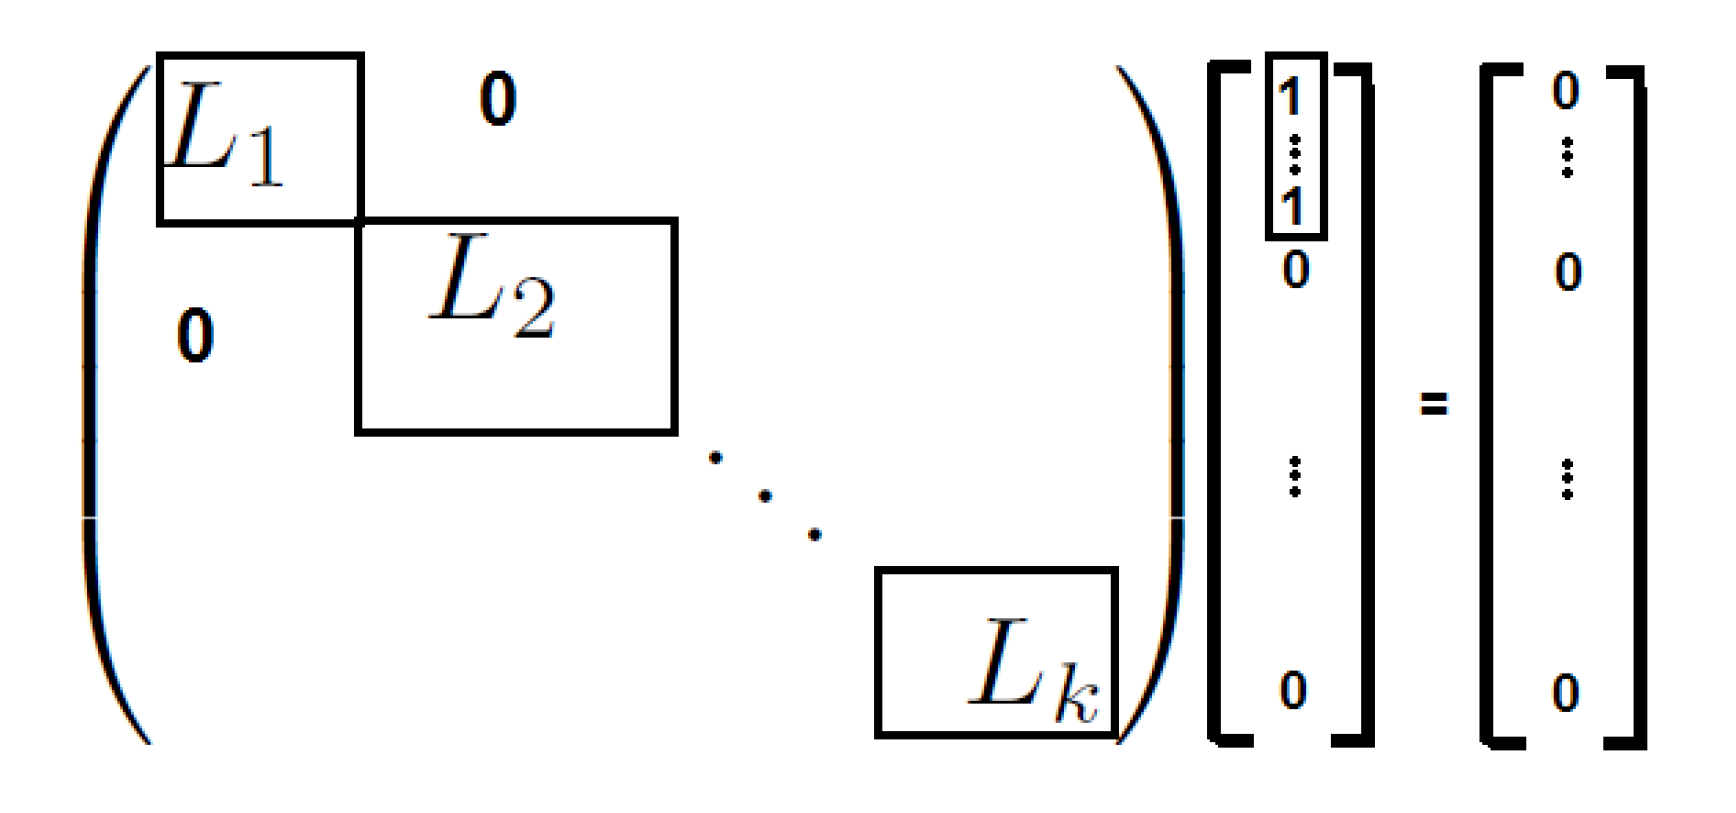
\includegraphics[scale=0.3]{Images/Laplacian.png}
	\caption{بردار ویژه متناظر با مقدار ویژه صفر در ماتریس لاپلاسین گراف دارای $k$ مولفه همبند} \label{Fig Laplacian}
\end{figure}

	\item گراف همبند که دارای یک مولفه همبندی است، تنها یک مقدار ویژه برابر با صفر دارد که بردار متناظر با آن برداری است که تمام المان‌های آن 1 باشد.

\end{enumerate}

حال که خواص ماتریس لاپلاسین بررسی شد، در قسمت بعد پایداری رابطه \ref{eq x. = -Lx} اثبات می‌گردد.

\newpage
\subsection{پایداری کنترل اجماع}
در کنترل اجماع، موقعیت عامل رهبر، $x_m$، به سیستم وارد می‌شود و کنترل اجماع تاثیری بر روی آن ندارد و $_l\dot{x}$ از طریق الگوریتم مسیریابی تعیین می‌گردد. لذا در رابطه \ref{eq x. = -Lx} سطر اول $L$ برابر صفر می‌گردد. به عنوان مثال در این پروژه، $L$ جدید، طبق رابطه \ref{eq L example} برابر است با:
\begin{equation}
L = 
\begin{bmatrix}
0~~~~~~0~~~~~~~0~~~~~~0 \\
-1~~~~~~3~~~-1~~~-1 \\
-1~~~-1~~~~~~3~~~-1 \\
-1~~~-1~~~-1~~~~~~3
\end{bmatrix}
\end{equation}

اگر $x$ برای مسئله یک رهبر و $n$ عامل دیگر به صورت زیر تعریف گردد:
\begin{equation}
x = 
\begin{bmatrix}
x_m \\
x_1 \\
x_2 \\
\vdots \\
x_n
\end{bmatrix}
\end{equation}

می‌توان $x_m$ را به صورت ورودی سیستم در نظر گرفت و سیستم را به شکل زیر بازنویسی کرد:
\begin{equation}\label{eq platoon system}
	\dot{x} = Ax + Bu, u = x_m
\end{equation}

که در آن $A$ و $B$ به شکل زیر از روی درایه‌های ماتریس $L$ به دست می‌آیند:
\begin{equation}\label{eq platoon AB}
A = 
\begin{bmatrix}
l_{22}~l_{23}~\cdots~l_{2n} \\
l_{32}~l_{33}~\cdots~l_{3n} \\
~~~~~~~~~\vdots~~~~~~~~~\\
l_{n2}~l_{n3}~\cdots~l_{nn} 
\end{bmatrix}
, B = 
\begin{bmatrix}
l_{21}\\
l_{31}\\
\vdots\\
l_{n1} 
\end{bmatrix}
\end{equation}

چون ماتریس اولیه لاپلاسین بوده پس اگر مقادیر هر سطر $B$ را از درایه قطر اصلی ماتریس $A$ که همان درایه قطر اصلی ماتریس لاپلاسین اولیه است کم کنیم به یک ماتریس لاپلاسین می‌رسیم. از اینجا به بعد منظور از ماتریس $L$ ماتریسی است که در تعریف زیر آمده است.
\begin{equation}\label{eq ABL relation}
	A + diag(B) = -L,~ diag(B) = 
	\begin{bmatrix}
	B_1~~0~~\cdots~~~~0 \\
	0~~~B_2~\cdots~~~0 \\
	~~~\vdots~~~\\
	~0~~~~0~~\cdots~~B_n
	\end{bmatrix}
\end{equation}

همچنین در ادامه منظور از ماتریس $\mathbbm{1}$ ماتریسی است که تمام درایه‌های آن 1 باشند.

ماتریس خطا، $e$، به صورت زیر تعریف می‌شود:
\begin{equation}\label{eq e definition}
	e = x - \mathbbm{1}x_m
\end{equation}

به کمک روابط \ref{eq platoon system} و \ref{eq ABL relation} داریم:
\begin{equation}\label{eq stability proof temp}
\dot{x} = Ax + Bx_m = -Lx - diag(B) + Bx_m
\end{equation}

با ادغام روابط \ref{eq stability proof temp} و \ref{eq e definition} می‌توان نوشت:
\begin{equation}
\dot{x} = -Le + L\mathbbm{1}x_m - diag(B)e
\end{equation}

با توجه به رابطه \ref{eq L1 = 0}، رابطه بالا به صورت زیر تبدیل می‌گردد:
\begin{equation}\label{eq x. = -Le -Be}
\dot{x} = -Le - diag(B)e
\end{equation}

که با کمک از رابطه \ref{eq ABL relation} می‌توان به رابطه زیر رسید:
\begin{equation}
	\dot{x} = Ae
\end{equation}

در نهایت چون بر متغیر $\dot{x}_m$ کنترلی نداریم و قرار است مطابق الگوریتم مسیریابی مقدار گیرد، آن را در هر فریم موقعیت عامل رهبر را ثابت می‌گیریم و در نتیجه می‌توان از مشتق آن صرف نظر کرد. با این فرض، سیستم دارای اندکی تاخیر می‌شود ولی در ادامه با اثبات پایدار مجانبی فراگیر\LTRfootnote{Globally asymptotically stable} بودن سیستم، مطمئن خواهیم بود که هنگام توقف خطا صفر خواهد بود. در نتیجه فرض بالا داریم:
\begin{equation}\label{eq x. = e.}
	\dot{x} = \dot{e}
\end{equation}

با استفاده از دو رابطه \ref{eq x. = -Le -Be} و \ref{eq x. = e.} نتیجه می‌شود:
\begin{equation}\label{eq dot e}
	\dot{e} = -Le -diag(B)e
\end{equation}

حال تابع کاندید لیاپانوف\LTRfootnote{Lyapunov candidate function}، $V(e)$، به صورت زیر تعریف می‌گردد، 
\begin{equation}\label{eq V definition}
V(e) = \frac{1}{2}e^Te > 0
\end{equation}

مشتق آن برابر است با:
\begin{equation}\label{eq V. = ee.}
\dot{V}(e) = e^T\dot{e}
\end{equation}

با جایگذاری رابطه \ref{eq dot e} در \ref{eq V. = ee.} خواهیم داشت:
\begin{equation}\label{eq V.}
\dot{V}(e) = -e^TLe - e^Tdiag(B)e
\end{equation}

حال به بررسی رابطه \ref{eq V.} می‌پردازیم. اولا طبق خواص مطرح شده در قسمت \ref{sec laplacian properties} و ماتریس مثبت معین بودن هر ماتریس لاپلاسینی داریم:
$\forall x,L~~x^TLx \ge 0$
 
در نتیجه در رابطه \ref{eq V.} داریم:
\begin{equation}\label{eq -ele<0}
	-e^TLe \le 0
\end{equation}

از طرفی با توجه به تعریف درایه‌های $B$ در رابطه \ref{eq platoon AB} که هیچ‌ یک درایه‌های قطر اصلی ماتریس لاپلاسین نیستند، درایه‌های $B$ می‌توانند یا صفر و یا یک باشند ولی حداقل یک درایه یک داریم، زیرا گراف همبند است و باید از عامل رهبر ارتباطی با بقیه موجود باشد. لذا اگر اندیس عامل‌هایی را که با عامل رهبر در ارتباط اند در مجموعه $N$ نگهداری کنیم داریم:
\begin{equation}\label{eq -ebe<0}
	-e^Tdiag(B)e = -\sum_{\forall j \in N}^{}e^2_j \le 0
\end{equation}

در نتیجه با توجه به روابط \ref{eq V.}، \ref{eq -ele<0} و \ref{eq -ebe<0} داریم:
\begin{equation}\label{eq V<0}
	\dot{V}(e) \le 0
\end{equation}

حال اثبات می‌کنیم که سیستم بالا پایدار مجانبی فراگیر است.

\begin{theorem}\label{th g.a.stable}
سیستم پایدار مجانبی است، اگر تنها یک نقطه تعادل پایدار داشته و تابع اسکالر $V(e)$ وجود داشته باشد که شرایط زیر را برآورده سازد:
\begin{enumerate}
	\item $V(e)$ در تمامی فضای حالت پیوسته و مشتق‌های جزئی پیوسته دارد.
	\item $V(e) > 0$ برای $x \ne 0$
	\item $V(0) = 0$
	\item $V(e) \to \infty$ به ازای $\|x\| \to \infty$
	\item $\dot{V}(e) \le 0$
و پاسخ غیر صفر 
$\dot{V}(e) = 0$
پاسخی از معادله دیفرانسیل سیستم نیست.
\end{enumerate}
\end{theorem}

شرایط 1 تا 4 توسط رابطه \ref{eq V definition} به دست می‌آیند. قسمت اول شرط 5، در رابطه \ref{eq V<0}
به دست آمده است. در ادامه قضیه \ref{th V. = 0} را اثبات می‌کنیم.

\begin{theorem}\label{th V. = 0}
اگر $e \ne 0$ وجود داشته باشد به طوری که $\dot{V} = 0$ باشد، آنگاه پاسخی از معادله دیفرانسیل سیستم نیست.

\end{theorem}

با برهان خلف قضیه را اثبات می‌کنیم. فرض خلف: فرض می‌کنیم $e_j$ وجود دارد به ظوری که 
$\dot{V}(e) = 0$.
تا به الان از فرض مهمی که در اثبات پایداری استفاده نشده است، همبند بودن گراف است. گفته شد چون گراف باید همبند باشد، پس از عامل رهبر به حداقل یکی از عامل‌ها باید ارتباط مستقیم وجود داشته باشد. در نتیجه حداقل یکی از درایه‌های بردار $B$ برابر 1 است. یکی از آن درایه‌ها را انتخاب می‌کنیم 
$B_i = 0$.
با توجه به رابطه \ref{eq V.} اگر $e_i \ne 0$ باشد، آنگاه عبارت 
$-e^TBe < 0$
خواهد بود که به همراه \ref{eq -ele<0} نتیجه می‌دهد 
$\dot{V}(e) < 0$ 
و به تناقض می‌رسیم. در نتیجه 
$e_n = 0$
باید باشد.

حال چون 
$e \ne 0$
در نتیجه درایه‌ای همانند   
$e_j \ne 0$ 
وجود دارد. حال از روی اینکه 
$\dot{e} = 0$ 
یا در حالت کلی 
\begin{equation}
\forall i = 1,2,...,n ~~ \dot{e}_i = 0
\end{equation}
باشد به تناقض خواهیم رسید. چون گراف همبند است پس هیچ راسی دارای درجه صفر نیست، لذا تمام داریه‌های قطر اصلی ماتریس $A$ غیر صفر هستند. اگر فقط درایه 
$e_j \ne 0$
داشته باشیم، در نتیجه چون داریه قطر اصلی متناظر با سطر $j$ مخالف صفر است، 
$\dot{e}_j \ne 0$
می‌شود. پس اگر $W$ مجموعه‌ی اندیس تمامی عامل‌های غیر لیدر باشد آنگاه $J$ را کوچک‌ترین مجموعه‌ای در نظر می‌گیریم به طوری که  
$J \subset W $
 از اندیس‌ها باشد به طوری که 
\begin{equation}
	\forall j \in J~~ e_j \ne 0
\end{equation}

و نتیجه دهد 
$\dot{e} = 0$.

دلیل اینکه امکان ندارد 
$J = W$
باشد این است که باید
$e_y = 0$
باشد.

حال دو حالت داریم: یا تمامی $e_{ji}$ ها با هم برابرند یا حداقل یک جفت وجود دارند که با هم ارتباط مستقیم دارند و در آن یکی از دیگری بزرگتر است.

اگر تمامی $e_{ji}$ با هم برابر و دارای مقدار $c$ باشند، به معنی آن است که اگر یک بردار $z$ تشکیل دهیم که متناظر با سطر $ji$ مقدار $c$ و در بقیه سطرها مقدار صفر بگیرد
$e = z$
، طبق رابطه \ref{eq dot e} داریم:
\begin{equation}\label{eq e. = -Lz - Bz}
	\dot{e} = -Lz~~-diag(B)z = 0
\end{equation}

و چون سطرهایی که $B_i = 1$ است، 
$z_i = 0$
است، خواهیم داشت:
\begin{equation}\label{eq Bz = 0}
	diag(B)z = 0
\end{equation}

با ادغام روابط \ref{eq e. = -Lz - Bz} و \ref{eq Bz = 0} داریم:
\begin{equation}
	Lz = 0
\end{equation}

که نتیجه می‌دهد $z$ بردار ویژه $L$ است و چون 
$z \ne \mathbbm{1}$
پس $L$ حداقل 2 مقدار ویژه مخالف صفر دارد که این با همبند بودن گراف اجماع در تناقض است. در نتیجه برای اینکه حالت بالا پیش نیاید جفت 
$|e_{j2}| > |e_{j1}|$
در مجموعه $J$ وجود دارند که دارای ارتباط مستقیم هستند.

نکته قابل توجه این است که در سطرهای عناصر $J$، درایه قطر اصلی برابر منفی مجموع درایه‌های دیگر است. در نتیجه اگر قدرمطلق درایه قطر اصلی در سطر $i \in J$ برابر $k_i$ باشد داریم:
\begin{equation}\label{eq sum in row}
	k_i e_{i} = \sum_{t \in T_i}^{}e_{t},~~ |T_i| = k_i
\end{equation}

که در آن $T_i$ مجموعه $t$هایی در سطر $i$ است که 
$a_{it} = 1$
باشد.

حال اگر سطر $j2$ را در نظر بگیریم، با توجه به رابطه \ref{eq sum in row} و 
$j1 \in T_{j2}$
داریم:
\begin{equation}\label{eq e > e}
\exists j3 \in T_{j2}~~|e_{j3}| > |e_{j2}|
\end{equation}

رابطه \ref{eq e > e}، مرنبا تکرار می‌شود و به $e_{j4}$ و بقیه $e_{ji}$ ها می‌رسیم. در نهایت چون یک رابطه خوش‌ترتیبی بیان گشته و مجموعه $W$ و در نتیجه آن $J$ متناهی است، عضوی همانند $e_jx$ وجود دارد که عضوی بزرگتر از اندازه آن در $J$ و چون بقیه‌ $e_i$ ها نیز برابر صفر هستند، عضوی بزرگتر از اندازه آن در بین کل $e_i$ها وجود ندارد. همچنین چون 
\begin{equation}\label{eq ejk-1 < ejx}
\exists j(x-1) \in T_{jx}~~s.t.~~|e_{j(x-1)}| < |e_{j(x)}|
\end{equation}

طبق رابطه \ref{eq sum in row} در سطر $jx$ داریم:
\begin{equation}\label{eq sum in row jx}
k_{jx} e_{jx} = e_{j(x-1)} + \sum_{t \ne j(x-1) \in T_{jx}}^{}e_{t},~~ |T_{jx}| = k_{jx}
\end{equation}

اگر از دو طرف رابطه \ref{eq sum in row jx}، قدرمطلق بگیریم داریم:
\begin{equation}\label{eq sum || in row jx}
k_{jx} |e_{jx}| = |e_{j(x-1)}| + \sum_{t \ne j(x-1) \in T_{jx}}^{}|e_{t}|,~~ |T_{jx}| = k_{jx}
\end{equation}

که با در نظر گرفتن روابط \ref{eq ejk-1 < ejx} و \ref{eq sum || in row jx}، نتیجه می‌شود که 
\begin{equation}
\exists t \in T_{jx}~~s.t.~~|e_t|>|e_jx|
\end{equation}

و این عبارت تناقض است.

در نتیجه تمامی شرایطی که در نظر گرفتیم، به تناقض رسید، پس فرض خلف باطل و حکم که قضیه \ref{th V. = 0} است، ثابت می‌گردد.

در نتیجه تمامی شرایط قضیه \ref{th g.a.stable} برقرار می‌گیرد و سیستم پایدار مجانبی فراگیر خواهد بودو خطا به صفر خواهد رسید.

\subsection{روش شکل‌دهی}
با رابطه \ref{eq x. = -Lx} به این رسیدیم که اگر یکی از عامل‌ها را رهبر در نظر بگیریم، بقیه آن را دنبال خواهند کرد. حال با یک حقه، ماتریس شکل‌دهی\LTRfootnote{formation} را تعریف و اعمال می‌کنیم. نسبت اختلاف موقعیت هر ربات را در $F$ که ماتریس شکل‌دهی است، قرار می‌دهیم و با رابطه \ref{eq x. = -L(x-f)}، کاری می‌کنیم که موقعیت واقعی عامل $i$ با اختلاف $F_i$ دیده شود و در نتیجه وقتی عامل میخواهد به موقعیت مطلوب $x_{di}$ برود در واقعیت به موقعیت $x_{di} + F_i$ خواهد رسید که همان هدف ما از شکل‌دهی است.
\begin{equation}\label{eq x. = -L(x-f)}
	\dot{x} = -L(x-F)
\end{equation} 

همچنین چون در دو بعد $x-y$ مشغول به کار هستیم، بردار $x$ را به ماتریس با دو ستون تغییر دادیم به طوری که یک ستون مربوط به فاصله در محور $x$ و یک ستون مربوط به فاصله در محور $y$ باشد. و در نتیجه ماتریس شکل‌دهی نیز دارای 2 ستون است.
\begin{equation}\label{eq X = [x y]}
	X = 
	\begin{bmatrix}
	x_1~~ y_1 \\
	x_2~~ y_2 \\
	\vdots \\
	x_n ~~y_n
	\end{bmatrix}
\end{equation}

\section{شبیه‌سازی و نتایج}





